%%%%%%%%%%%%%%%%%%%%%%%%%%%%%%%%%%%%%%%%%
% Two Column Curriculum Vitae XeLaTeX Template
%
% This template has been downloaded from:
% http://www.latextemplates.com
%
% Original author:
% Alessandro (The CV Inn)
%
% Modified by:
% Allen Zheng 2013-01-18
%
% IMPORTANT: THIS TEMPLATE NEEDS TO BE COMPILED WITH XeLaTeX
%
% This template uses several fonts not included with Windows/Linux by
% default. If you get compilation errors saying a font is missing, find the line
% on which the font is used and either change it to a font included with your
% operating system or comment the line out to use the default font.
% 
%%%%%%%%%%%%%%%%%%%%%%%%%%%%%%%%%%%%%%%%%

%----------------------------------------------------------------------------------------
%	PACKAGES AND OTHER DOCUMENT CONFIGURATIONS
%----------------------------------------------------------------------------------------

\documentclass[10pt]{article} % Font size (10pt, 11pt or 12pt)

\usepackage[hmargin=1.25cm, vmargin=1.5cm]{geometry} % Document margins

\usepackage{marvosym} % Required for symbols in the colored box
\usepackage{ifsym} % Required for symbols in the colored box

\usepackage[usenames,dvipsnames]{xcolor} % Allows the definition of hex colors

% Fonts and tweaks for XeLaTeX
\usepackage{fontspec,xltxtra,xunicode}
\defaultfontfeatures{Mapping=tex-text}
\setromanfont[Mapping=tex-text]{Hoefler Text} % Main document font use to English text.
\newfontfamily\zh{AR PL UKai CN} % Use AR PL UKai CN as chinese font
%\setsansfont[Scale=MatchLowercase,Mapping=tex-text]{Gill Sans MT Pro} % Font for your name at the top
%\setmonofont[Scale=MatchLowercase]{Andale Mono}
\newfontfamily\jl{xjlFont.ttf}
% Box used in interests section which follow up the weibo and QQ, it is fun.
\usepackage{fancybox}

% Colors for links, text and headings
\usepackage{hyperref}
\definecolor{linkcolor}{HTML}{506266} % Blue-gray color for links
\definecolor{shade}{HTML}{F5DD9D} % Peach color for the contact information box
\definecolor{text1}{HTML}{2b2b2b} % Main document font color, off-black
\definecolor{headings}{HTML}{701112} % Dark red color for headings
% Other color palettes: shade=B9D7D9 and linkcolor=A40000; shade=D4D7FE and linkcolor=FF0080

\hypersetup{colorlinks,breaklinks, urlcolor=linkcolor, linkcolor=linkcolor} % Set up links and colors

\usepackage{fancyhdr}
\pagestyle{fancy}
\fancyhf{}
% Headers and footers can be added with the \lhead{} \rhead{} \lfoot{} \rfoot{} commands
% Example footer:
%\rfoot{\color{headings} {\sffamily Last update: \today}. Typeset with Xe\LaTeX}

\usepackage{xcolor}
\newcommand{\blue}[1]{\textcolor{blue}{#1}}  % Defint the text color used in later and the color is blue

\renewcommand{\headrulewidth}{0pt} % Get rid of the default rule in the header

\usepackage{titlesec} % Allows creating custom \section's

% Format of the section titles
\titleformat{\section}{\color{headings}
\scshape\Large\raggedright}{}{0em}{}[\color{black}\titlerule]

\titlespacing{\section}{0pt}{0pt}{5pt} % Spacing around titles

\begin{document}

\color{text1} % Sets the default text color for the whole document

%----------------------------------------------------------------------------------------
%	GLOBAL TITLE
%----------------------------------------------------------------------------------------
%\raggedright{\LARGE\zh{郑又鑫}}\\
%\raggedright{\color{headings}\fontspec[Variant = 2]{Zapfino} Curriculum {Vit\fontspec[Variant = 3]{Zapfino}\ae}}
%\raggedleft{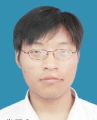
\includegraphics[scale=0.5]{touxiang.jpg}}
%\\[12pt]\par
	
%----------------------------------------------------------------------------------------

% Start the left-hand side of the page
\begin{minipage}[t]{0.5\textwidth}
\vspace{0pt} % Trick for alignmen

%---------------------------------------------------------------------------------------
%    SUB TITILE
%---------------------------------------------------------------------------------------

\raggedright{\Huge\zh{郑又鑫}\\[8pt]}
\raggedright{\color{headings}\fontspec[Variant = 2]{Zapfino} Curriculum {Vit\fontspec[Variant = 3]{Zapfino}\ae}\\[10pt]}


%----------------------------------------------------------------------------------------
%	WORK EXPERIENCE
%----------------------------------------------------------------------------------------

\section{\zh{工作经历}} 

%----------------------------------------------------------------------------------------
% WORK EXPERIENCE -1-

{\raggedleft\textsc{Mar 2012 -- Sep 2012}\par}

\raggedright{\large Morningstar.Inc (\zh{深圳})} \\
\raggedright{\textit{Equity Operation\\ QA Team Leader}\\[5pt]}

\normalsize{\zh{1.管理{\rmfamily QA}组日常工作,员工工作安排和考核.\\
                     2.改进质量控制逻辑并和开发部门合作实现更新.\\
                     3.定期撰写{\rmfamily Eqtuiy Data Product}的质量报告.\\
                     4.监控部门数据分析系统的状况并发送每日报告.\\
                     5.回复和解决客户的提交的产品问题.\\
                     6.参与了部门数个项目工作以及部门{\rmfamily BI}的初步设计.\\
                     7.组织多次针对员工的{\rmfamily SQL\& Excel}培训和知识分享活动.
                     }}\\[2pt]

%----------------------------------------------------------------------------------------
% WORK EXPERIENCE -2-

{\raggedleft\textsc{Dec 2010 -- Mar 2012}\par}

\raggedright{\large Morningstar.Inc (\zh{深圳})} \\
\raggedright{\textit{Equity Operation\\ Data Team Leader}\\[5pt]}

\normalsize{\zh{1.负责{\rmfamily Equity Data Team \uppercase\expandafter{\romannumeral6}}的日常工作.\\
                      2.特定行业上市公司财务数据跟踪分析.\\
                      3.监控美国市场{\rmfamily IPO}情况,负责{\rm IPO}数据分析.\\
                      4.管理{\rm Capital Structure}公司信用分析工作.\\
                      5.完成了新的{\rm IPO}和{\rm CS}平台的业务逻辑设计,开发和测试.
                      6.组织部门的{\rm SQL\&Excel}以及金融知识培训和知识分享活动.
                      }}\\[2pt]

%----------------------------------------------------------------------------------------
% WORK EXPERIENCE -3-

{\raggedleft\textsc{Dec 2009 -- Dec 2010}\par}

\raggedright{\large Morningstar.Inc (\zh{深圳})} \\
\raggedright{\textit{Equity Operation \\Data Analyst}\\[5pt]}

\normalsize{\zh{1.跟踪并及时收集上市公司公开发布的财务数据.\\
                      2.审核财务数据并根据既定的分析方法分析和挖掘财务数据.\\
                      3.检查计算后的财务数据指标是否合理.\\
                      4.负责特定行业的行业数据分析并研究行业分析方法.\\
                      5.参与一些研究项目和系统测试工作.
                      }}\\[2pt]

%----------------------------------------------------------------------------------------
% WORK EXPERIENCE -4-

{\raggedleft\textsc{\rm July 2009 -- Nov 2009}\par}

\raggedright{\large\rm ChinaScope Financial.Ltd (\zh{上海})}\\
\raggedright{\textit{Equity Research \\Financial Analyst}\\[5pt]}

\normalsize{\zh{1.跟踪上市公司撰写财务分析报告.\\
                      2.关注特定行业并撰写行业研究分析报告.\\
                      3.协助高级分析师,建立和完善财务分析估值模型.\\
                      4.完成其他工作.
                      }}\\[10pt]

%----------------------------------------------------------------------------------------	

%----------------------------------------------------------------------------------------
%  PROJECT EXPERIENCE
%----------------------------------------------------------------------------------------

\section{\zh{项目经验}} 

\begin{tabular}{rl}
2011.6 -- 2011.11&\textsl{Key Performance Indicators}\\[2pt]
2011.9 -- 2012.4&\textsl{Lean -- Financial Data Completeness}\\[2pt]
2011.12 -- 2012.5&\textsl{Equity Data API Testing}\\[2pt]
2011.6 -- 2011.9&\textsl{Capital Structure Design}\\[2pt]
&\\

\end{tabular}\\

%---------------------------------------------------------------------------------------
\end{minipage} % End left-hand side of the page
\hfill
% Start the right-hand side of the page
\begin{minipage}[t]{0.44\textwidth} 
\vspace{0pt} %trick for alignment

%----------------------------------------------------------------------------------------
%   PICTURE
%----------------------------------------------------------------------------------------

\raggedleft{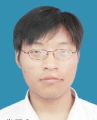
\includegraphics[scale=0.5]{touxiang.jpg}}
%----------------------------------------------------------------------------------------
%	COLORED BOX
%----------------------------------------------------------------------------------------
\section{\zh{联系信息}}

\colorbox{shade}{\textcolor{text1}{
\begin{tabular}{c|p{7cm}}
\raisebox{-3pt}{\textifsymbol{18}} & \zh{广东-深圳-罗湖} \\ % Address
\raisebox{-2pt}{\Mobilefone} & +86 180 2534 0388 \\ % Phone number
\raisebox{-0pt}{\Letter} & \href{mailto: zheng.youxin@gmail.com}{zheng.youxin@gmail.com} \\ % Email address
%\Keyboard & \href{http://www.johnsmith.com}{http://www.johnsmith.com} \\ % Website
\end{tabular}
}
}\\[10pt]

%----------------------------------------------------------------------------------------
%	EDUCATION
%----------------------------------------------------------------------------------------

\section{\zh{教育经历}} 

\begin{tabular}{rl} 

%----------------------------------------------------------------------------------------
% EDUCATION 
2005.9 -- 2009.7 & \textsc{\zh{南京财经大学}} \\
{} & \textsc{\zh{金融学}} \\ 
\zh{毕业论文} & \textsc{\zh{基于{\rm GRACH}的上证综指波动率研究}}\\
&\\

	 
%----------------------------------------------------------------------------------------

\end{tabular}\\[10pt]

%----------------------------------------------------------------------------------------
%	INTRODUCTION
%----------------------------------------------------------------------------------------

\section{\zh{个人简介}}

\begin{center}
\vspace{10pt}
\zh{爱}\raisebox{0.5ex}[12pt]{\jl{\blue{\Large 折腾}}},\zh{不爱}\raisebox{0.5ex}[12pt]{\jl{\blue{\Large 太消停}}}.\\[2pt]
\zh{爱}\raisebox{0.5ex}[12pt]{\jl{\blue{\Large 分析}}},\zh{不爱}\raisebox{0.5ex}[12pt]{\jl{\blue{\Large 无证立论}}}.\\[2pt]
\raisebox{0.5ex}[12pt]{\jl{\blue{\Large 金融}}}\zh{是我的专业}.\\[2pt]
\raisebox{0.5ex}[12pt]{\jl{\blue{\Large 技术}}}\zh{是我的兴趣和爱好}.\\[2pt]
\zh{我还有}\raisebox{0.5ex}[12pt]{\jl{\blue{\Large 其它}}}\zh{的兴趣和爱好}.\\[2pt]
\zh{我不是屌丝}\raisebox{0.5ex}[12pt]{\jl{\blue{\Large 程序猿}}}.\\[2pt]
\zh{也不是}\raisebox{0.5ex}[12pt]{\jl{\blue{\Large 金融高富帅}}}.\\[2pt]
\zh{专注}\raisebox{0.5ex}[12pt]{\jl{\blue{\Large 金融数据}}}\zh{三年}.\\[2pt]
\zh{只为了}\raisebox{0.5ex}[12pt]{\jl{\blue{\Large 金融风险管理}}}\zh{梦想}.\\[2pt]
\zh{要让投资者的资产}\raisebox{0.5ex}[12pt]{\jl{\blue{\Large 更安全}}}.\\[2pt]
\zh{就让}\raisebox{0.5ex}[12pt]{\jl{\blue{\Large 数据会说话!}}}\\[2pt]
\zh{这就是}\raisebox{0.5ex}[12pt]{\jl{\blue{\LARGE 我}}}.\\[2pt]
\zh{一个喜欢}\raisebox{0.5ex}[12pt]{\jl{\blue{\LARGE 互联网的金融男}}}.\\[5pt]

\end{center}
%---------------------------------------------------------------------------------------
%   INTERESTING LABLE
%--------------------------------------------------------------------------------------
\section{\zh{我的标签}}

\begin{tabular}{rl}
\zh{兴趣爱好} & \Ovalbox{\zh{体育}} \Ovalbox{\zh{历史}} \Ovalbox{\zh{武侠}} \Ovalbox{\zh{吉它}}  \Ovalbox{\zh{公益}} \Ovalbox{\zh{足球}}\\[5pt]
              & \Ovalbox{\rm Python} \Ovalbox{\rm DOTA} \Ovalbox{\rm Linux} \Ovalbox{\rm Emacs} \Ovalbox{\zh{摄影}}\\[5pt]
\zh{职业目标} & \Ovalbox{\zh{风险管理师}} \Ovalbox{\zh{产品经理}}\\[5pt]
              & \Ovalbox{\zh{数据分析师}} \Ovalbox{\zh{项目经理}}\\[5pt]
              
\end{tabular}\\[6pt]
%----------------------------------------------------------------------------------------
%	COMPUTER SKILLS
%----------------------------------------------------------------------------------------

\section{\zh{工作技能}} 

\begin{tabular}{rl}
\zh{了解} & \textrm{R, Axure, Hadoop, Emacs, sed\&awk}\\[3pt]
\zh{一般} & \textrm{\LaTeX , Python, Shell, Oracle, Visio, Vim}\\[3pt]
\zh{熟悉} & \textrm{Linux, SQL, MySQL, Excel,Eviews}\\[3pt]
\zh{其它} & \textrm{CET 6,\zh{高效沟通}}\\[3pt]
&\\

\end{tabular}


%----------------------------------------------------------------------------------------
	
\end{minipage} % End right-hand side of the page
\end{document}  

